\chapter{Power Amplifiers}

In the previous chapter, we studied all kinds of amplifiers. However, we never looked at power amplification and how power was provided to the load resistance,  but we only were interested in amplification of the input voltage. In this chapter, we're mostly interested in power consumption and efficiency, and we'll look at amplifiers of class A, B, C, D and S. We'll also study current amplifiers like push-pull amplifiers, and selective amplifiers that only amplify signals around a central frequency.

\section{Introduction}
Until now, we were not concerned with power consumption or efficiency of the amplifiers we have studied. We only cared about achieving high gain. In this chapter, we look at \emph{power amplifiers}, amplifiers made to deliver power - and to do this as efficiently as possible.\\
First, we will consider a simple common emitter amplifier in figure \ref{fig:pa_circuit1}. Notice that we don't consider an emitter resistance $R_E$. This is because typically, $R_E$ is quite low; if not, the possible voltage swing along the dynamic load line would become too small.\\
With proper biasing and neglecting $V_{CE, Sat}$, we see that $V_{CEQ} = \frac{E}{2}$ and $I_{CQ} = \frac{E}{2R_C}$ so that $Q$ is nicely in the middle of the operating domain, as in figure \ref{fig:pa_circuit2}. The load line is given by $E = R_C \; i_c + v_{CE}$. Furthermore, we assume that the collector resistor $R_C$ is the load to which we want to deliver power.

\begin{minipage}{.5\textwidth}
	\centering
	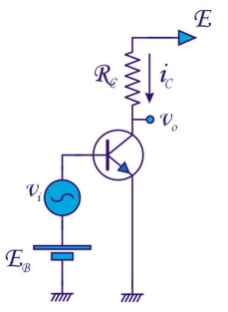
\includegraphics[height=6cm]{figures/ch09/pa_circuit1.jpg}
	\captionof{figure}{ }
	\label{fig:pa_circuit1}
\end{minipage}%
\begin{minipage}{.5\textwidth}
	\centering
	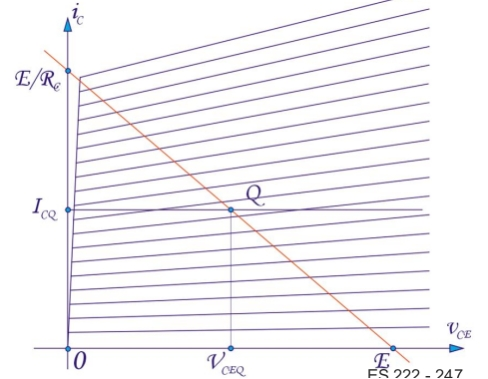
\includegraphics[width=8cm]{figures/ch09/pa_circuit2.jpg}
	\captionof{figure}{ }
	\label{fig:pa_circuit2}
\end{minipage}

We assume that the applied input signal $v_i$ is sinusoidal. If $E_B$ is large enough, the collector current $i_C$ will also be a sinusoid and the transistor is always conducting, as in the top of figure \ref{fig:pa_cycle1}. But if we decrease the input bias source $E_B$, $I_{CQ}$ can be reduced, and from a certain point on (namely when $E_B + v_i = V_{BEQ}$), $i_C$ will become equal to zero (figure \ref{fig:pa_cycle2} bottom), and can't become negative because the circuit can't conduct in the other direction. If $E_B$ decreases even further, the transistor will conduct less then half of the time (figure \ref{fig:pa_cycle2}).\\
The \emph{conduction angle} $\theta$ is defined as:
\begin{equation}
	\theta = \frac{T_{conduct}}{T} \times 180^{\circ} 
	\label{eq:condcution_angle}
\end{equation}
Based on the conduction angle, $4$ different classes of amplifiers are defined:
\begin{enumerate}
	\item Class A: $\theta = 180^{\circ} $
	\item Class AB: $90^{\circ} < \theta < 180^{\circ} $
	\item Class B: $\theta = 90^{\circ} $
	\item Class C: $\theta < 90^{\circ} $
\end{enumerate}


\begin{minipage}{.5\textwidth}
	\centering
	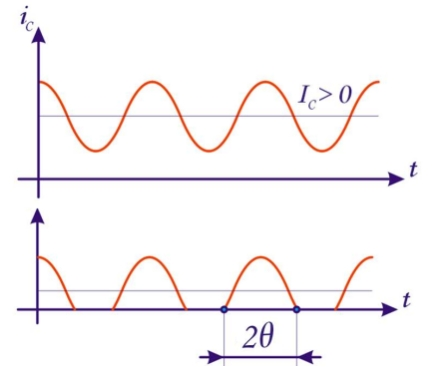
\includegraphics[width=7cm]{figures/ch09/pa_cycle1.jpg}
	\captionof{figure}{ }
	\label{fig:pa_cycle1}
\end{minipage}%
\begin{minipage}{.5\textwidth}
	\centering
	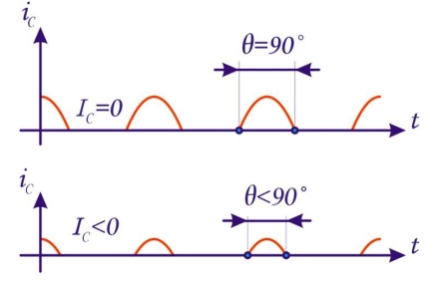
\includegraphics[width=7cm]{figures/ch09/pa_cycle2.jpg}
	\captionof{figure}{ }
	\label{fig:pa_cycle2}
\end{minipage}

In the rest of this chapter, we study a circuit for each type of conduction. We will compute the power efficiencies, by considering only the circuit on the collector side. All other power consumptions, like base currents or power consumed in the emitter (source) resistance will be neglected.\\
The instantaneous power consumed by an element in a circuit is $p(t) = v(t) i(i)$ with $v$ and $i$ the instantaneous voltage and current through the element. When the signals are sinusoidal, we define the average power dissipated during one period $T$:
$$
P = \frac{1}{T}\;\int_{t_0}^{t_0 + T} v(t) \; i(t) \; dt
$$

\section{Class A Amplifier}
\label{sec:classA}

We assume that the applied input signal $v_i$ is sinusoidal and thus:
\begin{align*}
	v_{CE} &= V_{CEQ} +  V_{cem} \sin(\omega t) = V_{CEQ}  + v_{ce}(t) \\
	i_C &= I_{CQ} - I_{cm} \sin(\omega t) = I_{CQ} + i_{c} (t)
\end{align*}
with $V_{cem} = R_C I_{cm}$.\\
Because $Q$ is located in the middle of the operating region, we also have $V_{CEQ} = E/2$ and $I_{CQ} = \frac{E}{2R_C}$.\ Consequently, the voltage and current amplitudes are limited to: $V_{cem} \le E/2$ and $I_{cem }\le \frac{E}{2R_C}$.\\
We calculate\footnote{Note that $\int_{0}^{T} \sin(\omega t) \; dt = 0$ and $\int_{0}^{T} \sin^2(\omega t) \; dt = \frac{T}{2}$}:
\begin{itemize}
	\item $P_D$, the power delivered to the circuit by the supply $E$:
	$$
	P_D = \frac{1}{T}\;\int_{t_0}^{t_0 + T} E \; i_C(t) \; dt = E\;I_{CQ} = \frac{E^2}{2 R_C}
	$$
	\item $P_C$, the power dissipated by the transistor:
	\begin{align*}	
	P_C &= \frac{1}{T}\;\int_{t_0}^{t_0 + T} v_{CE}(t) \; i_C(t) \; dt \\
		&= \frac{1}{T}\;\int_{t_0}^{t_0 + T} (V_{CEQ} +  V_{cem} \sin(\omega t)) \; (I_{CQ} - I_{cm} \sin(\omega t)) \; dt \\
		&=  \frac{1}{T}\;\int_{t_0}^{t_0 + T} (V_{CEQ}\;I_{CQ} -  V_{cem} \; I_{cm}\sin(\omega t)^2)\; dt \\
		&= V_{CEQ}\;I_{CQ} - \frac{1}{2}V_{cem} \; I_{cm}  = \frac{E^2}{4R_C} -\frac{1}{2}\frac{V_{cem}^2}{R_C} \\
		&= \frac{E^2}{4R_C} - \frac{1}{2}\frac{E^2}{4R_C}  = \frac{E^2}{8R_C} \text{ at $V_{cem} = E/2$ and $I_{cm}= \frac{E}{2R_C}$}
	\end{align*}
	\item $P_L$, the AC power delivered to the load $R_C$ because the only useful power delivered to the load is the variation of the signal around the average value. Note that $v_{R_C} + v_{ce} = 0$ and $i_{R_C} = i_c$. So:
	\begin{align*}	
		P_L &= \frac{1}{T}\;\int_{t_0}^{t_0 + T} v_{R_C}(t) \; i_{R_C}(t) \; dt  = \frac{1}{T}\;\int_{t_0}^{t_0 + T} v_{ce}(t) \; i_c(t) \; dt \\
			&= \frac{1}{2}V_{cem} \; I_{cm} \\
			&=\frac{1}{2}\frac{E^2}{4R_C} =\frac{E^2}{8R_C} \text{ at $V_{cem} = E/2$ and $I_{cm} = \frac{E}{2R_C}$}
	\end{align*}
	\item $P_J$, the rest:
	\begin{align*}
		P_J = P_D - P_C - P_L &= \frac{E^2}{2 R_C} - \bigg(\frac{E^2}{4R_C} -\frac{1}{2}\frac{V_{cem}^2}{R_C}\bigg) - \frac{1}{2}V_{cem} \; I_{cm} \\
							  &= \frac{E^2}{4R_C} = R_C I_{CQ}^2
	\end{align*}
\end{itemize}
This last term $P_J$ is caused by the DC current $I_{CQ}$ in the load resistor $R_C$.\\
The efficiency of the amplifier $\eta$ is defined as the ratio between power delivered to the load over the total power delivered by the supply:
\begin{equation}
	\eta = \frac{P_L}{P_D} = \frac{V_{cem}^2}{E^2}
\end{equation}
With $V_{cem, max} = \frac{E}{2}$ we find the maximum efficiency: $\eta_{max} = \frac{1}{4}$. The quality factor $F$ is the ratio between the maximum power consumed by the transistor $P_{C, max}$ and the maximum power consumed by the load $P_{L, max}$. The former happens when $V_{cem} = 0$ and is equal to: $P_{C, max} = \frac{E^2}{4R_C}$, the latter occurs at full swing $V_{cem} =E/2$ and is equal to  $P_{L, max} = \frac{E^2}{8R_C}$. Thus $$F = \frac{P_{C, max}}{P_{L, max}} = 2$$\\
\begin{figure}[h!]
	\centering
	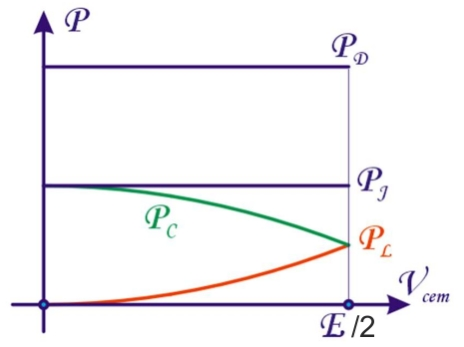
\includegraphics[width=6cm]{figures/ch09/pa_cycle3.jpg}
	\caption{Power distribution for increasing $V_{cem}$}
	\label{fig:pa_cycle3}
\end{figure}
These different power contributions are shown in figure \ref{fig:pa_cycle3} as a function of the voltage swing $V_{cem}$. Note how the maximum efficiency is only $25\%$, achieved at the maximal value of $V_{cem}$. Half the power $P_J = \frac{E^2}{8R_C} = R_C I_{CQ}^2$ is used to generate the bias current for the transistor, which also runs trough the load resistor $R_C$ but doesn't provide anything useful. This power is useless and should be eliminated to increase the efficiency $\eta$.\\
To improve this, we want to avoid any DC current in the load. We propose the circuit in figure \ref{fig:classA1}. If $L$ is very large, the inductor will be a short-circuit for DC signals. And if $C_L$ is very large, the load resistor $R_L$ is isolated from the bias currents. Thus $I_{CQ}$ doesn't flow through the load, in contrast with the previous situation. Consequently, $V_{CEQ} = E$ and $I_{CQ} = \frac{E}{R_C}$ and the operating point $Q$ is uniquely determined.\\
\begin{minipage}{.5\textwidth}
	\centering
	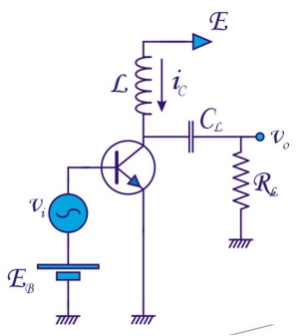
\includegraphics[width=6cm]{figures/ch09/classA1.jpg}
	\captionof{figure}{Class A Amplifier}
	\label{fig:classA1}
\end{minipage}%
\begin{minipage}{.5\textwidth}
	\centering
	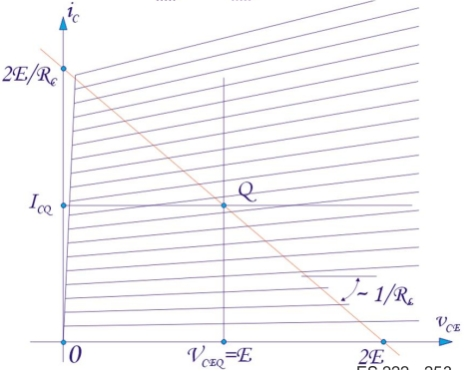
\includegraphics[width=9cm]{figures/ch09/classA2.jpg}
	\captionof{figure}{Load lines and Q-point}
	\label{fig:classA2}
\end{minipage}
For AC signals however, the inductor is an open circuit and $C_L$ is a short circuit, so we can write the dynamic load line: $v_{ce} = -R_L\; i_c$. The load lines (static in blue, dynamic in red) are sketched in figure \ref{fig:classA2}. Note how $v_{CE}$ can become higher then the power supply $E$. This is because the inductance will create an electromotive force (EMF) at the frequency we are working at to keep the current through it constant. This EMF can increase the voltage at the collector to $2E$. This also means that $V_{cem, max} = E$ and $I_{cem, max} = E/R_L$.\\
We can recompute the different powers:
\begin{itemize}
	\item $P_D = \frac{1}{T} \int_{t_0}^{t_0 + T} E \; i_C(t) dt = E \; I_{CQ} = \frac{E^2}{R_L}$
	\item $P_C = \frac{1}{T} \int_{t_0}^{t_0 + T} v_{CE}(t) \; i_C(t) \; dt = V_{CEQ}\;I_{CQ} - \frac{V_{cem}^2}{2R_L} = \frac{E^2}{2R_L}$
	\item $P_L =  \frac{1}{T} \int_{t_0}^{t_0 + T} v_{ce}(t) \; i_c(t) \; dt = \frac{V_{cem}^2}{2R_L} = \frac{E^2}{2R_L}$
\end{itemize}
Note how $P_C + P_L = P_D$ and thus $P_J = 0$. This is because there runs no DC (and hence useless) power through the load resistance. The different powers are shown in figure \ref{fig:classA3}.
\begin{figure}[h!]
	\centering
	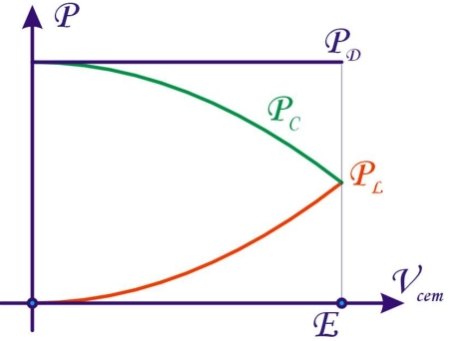
\includegraphics[width=6cm]{figures/ch09/classA3.jpg}
	\caption{Power distribution for class A amplifier}
	\label{fig:classA3}
\end{figure}
\\The efficiency $\eta = \frac{P_L}{P_D} = \frac{V_{cem}^2}{2E^2}$ so that $\eta_{max} = \frac{1}{2}$, and the quality factor $F = 2$. The maximum efficiency (reached at maximum amplitude) is thus $50\%$, instead of $25\%$ as before.
\subsection{Improvement to the class A amplifier}
This issue with the previous circuit is this: typically, the power supply $E$ is given, and when you buy a speaker, the internal resistance $R_L$ is also given. This means that the maximum power you can deliver to the load, namely $\frac{E^2}{2R_L}$ is also fixed, even though the speaker may have a higher $P_{L, max}$.\\
An alternative circuit to the one in figure \ref{fig:classA1} is the one in figure \ref{fig:classA4} where a transformer is used to transfer the AC power to the load and the conversion factor $n$ can be set. This additional degree of freedom will allow to increase the maximum power.\\
\begin{minipage}{.5\textwidth}
	\centering
	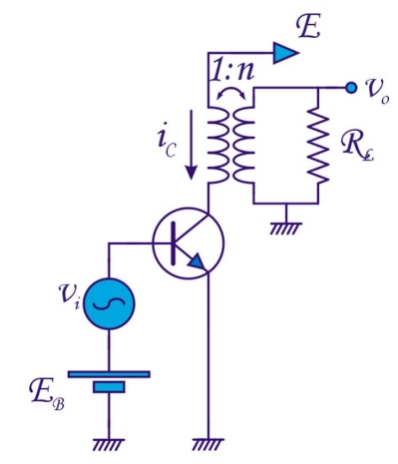
\includegraphics[width=6cm]{figures/ch09/classA4.jpg}
	\captionof{figure}{Improved Class A Amplifier}
	\label{fig:classA4}
\end{minipage}%
\begin{minipage}{.5\textwidth}
	\centering
	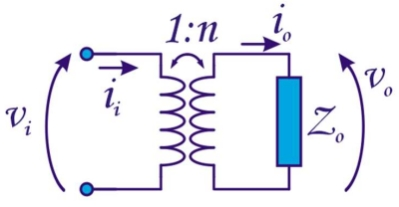
\includegraphics[width=7cm]{figures/ch09/classA5.jpg}
	\captionof{figure}{Transformer}
	\label{fig:classA5}
\end{minipage}
In this circuit, we have the same DC load line as before: $v_{CE} = E$, but the AC load line is now $v_{ce} = -R_L' \; i_e$ where $R_L'$ is the load as seen by the biasing circuit.\\
To understand this, consider the transformer in figure \ref{fig:classA5}. A transformer works by generating a changing magnetic field $\Phi_B(t)$ with an inductor. This flux flows then through another inductor which generates an EMF due to Faraday's law of induction: $\mathcal{E} = -\frac{d\Phi_B}{dt}$. Because a transformer only works for AC signals, the load seen by the DC circuit is zero - the transformer acts as a short-circuit. For AC signals however, as in figure \ref{fig:classA5}, the impedance $Z_i$ seen by the circuit is different. Because the relation between currents and voltages is:
\begin{align*}
	n \; I_o &= I_i \\
	V_o &= n \; V_i
\end{align*}
we find that $Z_i = \frac{V_i}{I_i} = \frac{V_o}{n^2 \; I_o} = \frac{Z_o}{n^2}$. This means that the load $R_L$ is reflected into the circuit and the circuit sees $R_L' = R_L/n^2$. For a given $E$, $R_L$ and $P_{L, max}$, we know for the reflected load (the apparent resistor) that $P_{L, max} = \frac{E^2}{2R_L'}$ and thus:
$$
R_L' = \frac{E^2}{2P_{L, max}}
$$
and from $R_L'$ and the true $R_L$, we find the turns ratio $n$:
$$
n = \sqrt{\frac{R_L}{R_L'}}
$$
In an audio amplifier, this turns ratio can often be set be turning a screw.
\section{Class B Amplifier}
\label{sec:classB}
In the class A amplifier from the previous section, there was always a current $I_{CQ}$ and a current variation $i_c$ around this value because there is a bias source $E_B$ that lifts the base voltage at the input transistor to a level that allows conduction in the right branch. This also means that the transistor dissipates power even when there is no signal ($V_{cem} = 0$) - it will even dissipate all power delivered to the circuit, which is constant.\\
We could remove this bias source, as in figure \ref{fig:classB1}. However, in that case there will only be a non-zero voltage of $R_L$ during half of the period, namely when $v_i > 0$, as in figure \ref{fig:classB2}. Note that the voltage is negative because the circuit has a negative gain.\\

\begin{minipage}{.5\textwidth}
	\centering
	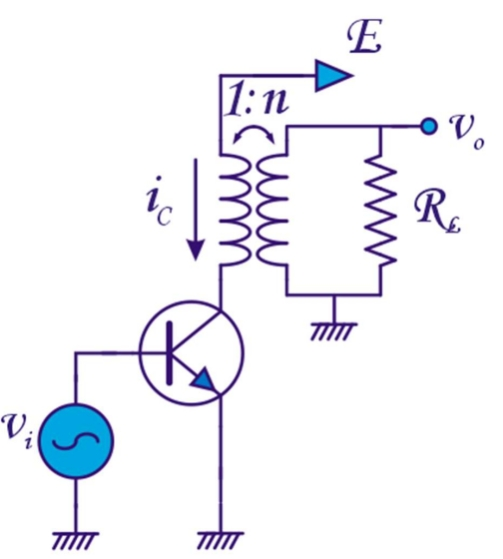
\includegraphics[width=5cm]{figures/ch09/classB1.jpg}
	\captionof{figure}{Class A Amplifier without $E_B$}
	\label{fig:classB1}
\end{minipage}%
\begin{minipage}{.5\textwidth}
	\centering
	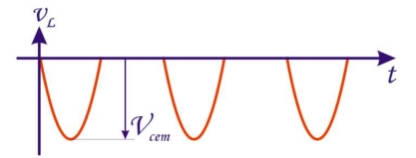
\includegraphics[width=7cm]{figures/ch09/classB2.jpg}
	\captionof{figure}{Signal produced in $R_L$}
	\label{fig:classB2}
\end{minipage}

This is off course not an acceptable situation, but we can create a signal during the entire period of the input signal by effectively putting two of these circuits on top of each other, as in figure \ref{fig:classB3}. Note that we use both $v_i$ and $-v_i$ and two npn-transistors with interconnected emitters and opposite base-emitter voltages. On the load side, note that the dots signify wether the turns of the inductors turn in the same direction or not. \\
Transistor \Circled{1} will conduct only when $v_i > 0$ and generates a signal of the form of figure \ref{fig:classB2} in $R_L$. Transistor \Circled{2} conducts only when $v_i < 0$ and generates the opposite signal of figure \ref{fig:classB2}. When both signals are added together, the complete wave form is restored. Note that we have neglected that $V_{BEQ} \approx 0.6$ V - we will come back to this later.\\
The DC load line for transistor \Circled{1} has the same expression as behavior: $v_{CE} = E$, but $I_{CQ} = 0$ because the transistor is blocked when $v_i = 0$. Thus the operating point lies on the x-axis of figure \ref{fig:classB4} and the dynamic load line with slope $-\frac{1}{R_L'}$ passes through this point. As $v_i$ increases, $v_{CE}$ of transistor \Circled{1} decreases because we move up the load line, as shown in figure \ref{fig:classB4}, until the maximum current $E/R_L'$ is reached. At the same time, transistor \Circled{2} is blocked but $v_{CE}$ of \Circled{2} increases from $E$ to $2E$ because the transformer induces an EMF from the right inductor to the inductor in the loop with the emitter-collector of transistor \Circled{2}. The $V_{CE}$ of \Circled{2} moves along the horizontal line from $Q$ to $2E$. When $v_i$ becomes negative, the situation is reversed for both transistors.

\begin{minipage}{.5\textwidth}
	\centering
	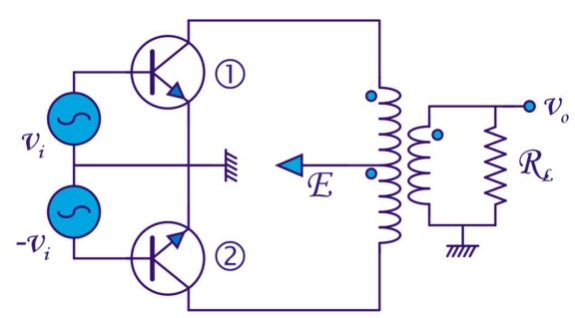
\includegraphics[width=7cm]{figures/ch09/classB3.jpg}
	\captionof{figure}{Class B Amplifier}
	\label{fig:classB3}
\end{minipage}%
\begin{minipage}{.5\textwidth}
	\centering
	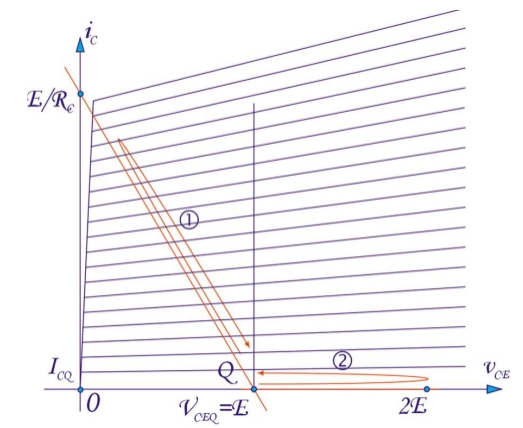
\includegraphics[width=7cm]{figures/ch09/classB4.jpg}
	\captionof{figure}{Load lines of figure \ref{fig:classB3}}
	\label{fig:classB4}
\end{minipage}
Let's compute the different powers, just as before. However, keep in mind that every transistor is only active half of the time, so we integrate during $T/2$ and multiply the result by two: %\footnote{Remember: $\int_0^{\pi} \sin(x) \; dx = 2$ and $\int_0^{\pi} \sin^2(x) \; dx = \pi/2$}: %(\textbf{TODO:} check results)
\begin{itemize}
	\item $P_D = 2 \frac{1}{T} \int_{t_0}^{t_0 + T/2} E \; I_{cm} \; \sin(\omega t) dt = \frac{2}{\pi} \; E \; I_{cm}  = \frac{2}{\pi}\frac{E\;V_{cem}}{R_L'} = \frac{2}{\pi}\frac{E^2}{R_L'}$
	\item $P_L = 2 \frac{1}{T} \int_{t_0}^{t_0 + T/2} V_{cem} \; I_{cm} \; \sin^2(\omega t) dt = \frac{V_{cem}^2}{2R_L'} = \frac{E^2}{2R_L'}$
	\item And consequently, since there is no power dissipated for biasing: \\
	$P_C = P_D - P_L = \frac{2}{\pi} \frac{E\; V_{cem}}{R_L'} - \frac{V_{cem}^2}{2 R_L'}$
\end{itemize}
We see that $P_D$ increases monotonically with the signal amplitude $V_{cem}$ (there was no dependence in the class A amplifier) - see figure \ref{fig:classB7}.

\begin{figure}[h!]
	\centering
	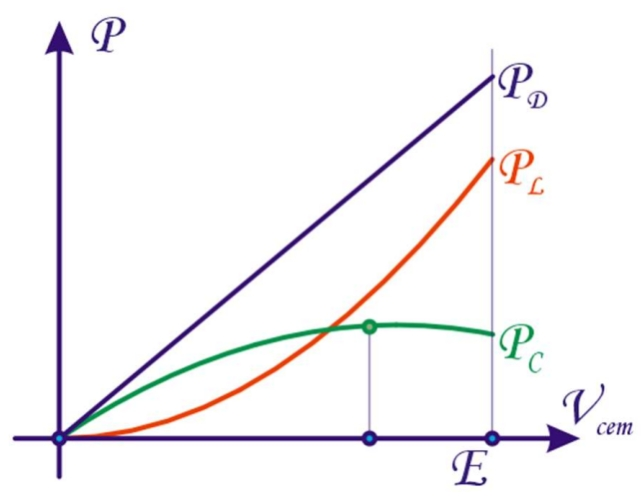
\includegraphics[width=6cm]{figures/ch09/classB7.jpg}
	\caption{Power distribution for class B amplifier}
	\label{fig:classB7}
\end{figure}

$P_C$ has a quadratic behavior and reaches a maximum when:
$$
\frac{dP_C}{dV_{cem}} =  \frac{2}{\pi} \frac{E}{R_L'} - \frac{V_{cem}}{R_L'} = 0
$$
this is at $V_{cem} = \frac{2}{\pi} E$ and thus 
$$P_{C, max} = P_C \big|_{V_{cem} = \frac{2E}{\pi}} = \frac{2E^2}{\pi^2 R_L'}$$
The efficiency $\eta$ is equal to:
$$
\eta = \frac{P_L}{P_D} = \frac{\pi}{4} \frac{V_{cem}}{E} 
$$
and $\eta_{max} = \frac{\pi}{4}$. In other words, the maximum efficiency, reached when $V_{cem} = V_{cem, max} = E$, is about $78\%$. The quality factor $F$ is:
$$F = \frac{P_{C, max}}{P_{L, max}} = \frac{2E^2}{\pi^2 R_L'} / \frac{E^2}{2R_L'} =   \frac{4}{\pi^2}$$

and for each transistor $F_{Tr} = \frac{2}{\pi^2}  \approx 0.2$. So for every $5$ W delivered to the load, the transistor consumes only $1$ W. This is a lot better then before.
\subsubsection{How to generate $-v_i$\;?}
Given $v_i$, there are basically two ways te generate $-v_i$, as required by the class B amplifier:
\begin{enumerate}
	\item By using a phase splitter, i.e. an amplifier with $R_C = R_E$, where the outputs are taken at the collector (180° out-of-phase) and at the emitter (in-phase), as in figure \ref{fig:classB9}.
	\item By using a transformer, as in figure \ref{fig:classB8}.
\end{enumerate}

\begin{minipage}{.5\textwidth}
	\centering
	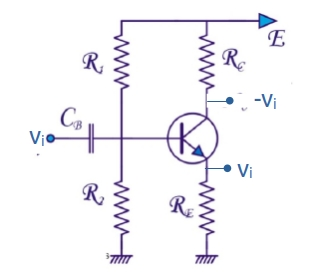
\includegraphics[width=5cm]{figures/ch02/phase_splitter.jpg}
	\captionof{figure}{}
	\label{fig:classB9}
\end{minipage}%
\begin{minipage}{.5\textwidth}
	\centering
	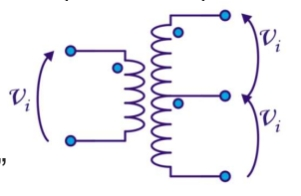
\includegraphics[width=6cm]{figures/ch09/classB8.jpg}
	\captionof{figure}{}
	\label{fig:classB8}
\end{minipage}

\subsubsection{What if $V_{BEQ} \ne 0$?}
Until now, we have neglected the threshold voltage $V_{BEQ}$ needed to generate a current in the transistor. But in reality, $v_i > 0.6$ V before the transistor conducts. If we take this into account, the resulting current waveform is not a perfect sinusoid, but rather a cascade of half-periods interrupted by regions of zero current, when $v_i$ is too low to generate a forward bias in the base-emitter junctions, as in figure \ref{fig:classB6}. This phenomenon is called \emph{cross distortion}.\\
\begin{minipage}{.5\textwidth}
	\centering
	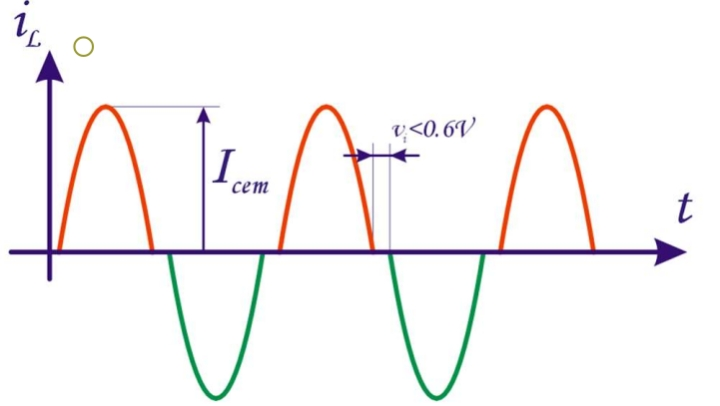
\includegraphics[width=7cm]{figures/ch09/classB6.jpg}
	\captionof{figure}{}
	\label{fig:classB6}
\end{minipage}%
\begin{minipage}{.5\textwidth}
	\centering
	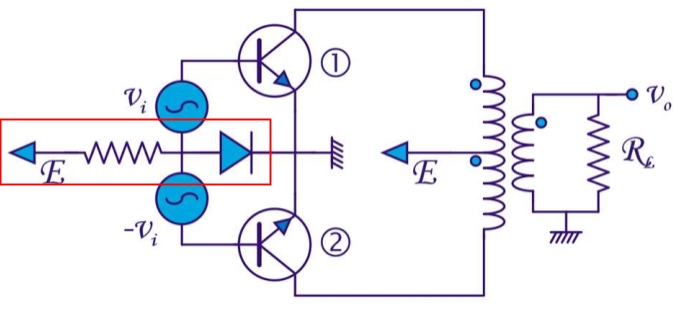
\includegraphics[width=7cm]{figures/ch09/classB5.jpg}
	\captionof{figure}{}
	\label{fig:classB5}
\end{minipage}
A way to solve this is to pre-bias the loop with the base-emitter junction, by adding one threshold voltage via a diode, as in figure \ref{fig:classB5} - the part in red is the pre-bias circuit. This circuit adds one $V_{BEQ}$ to $v_i$ such that a positive $v_i$ is enough to generate a collector current in transistor \Circled{1} because the voltage at its base will be $v_i + 0.6$ V.

\section{Push-Pull Amplifiers}
\label{sec:push_pull}
A similar idea of using two transistors circuits on top of each other, is the so-called \emph{push-pull} topology of figure \ref{fig:pushpull1}. The goal is not to amplify a voltage, but to deliver current to and from a load $R_L$.\\
The circuit consists of an input voltage $v_i$ that will be coupled in through capacitors $C_B$, two biasing circuits with resistors $R_B$ and $R$ that put the base voltage at $\frac{R_B R}{R_B + R} E$, and two transistors in common-collector configuration (i.e. as emitter followers). Note that transistor \Circled{1} is an npn, but \Circled{2} is a pnp transistor. The load $R_L$ is thus connected to the emitters of both transistors.\\
\begin{minipage}{.5\textwidth}
	\centering
	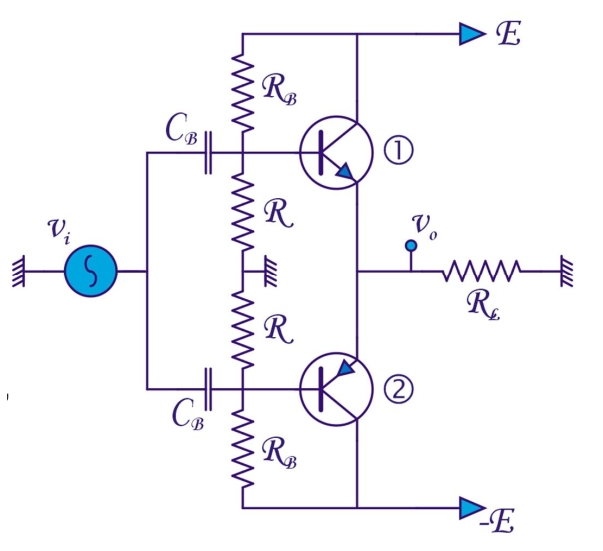
\includegraphics[width=8cm]{figures/ch09/pushpull1.jpg}
	\captionof{figure}{}
	\label{fig:pushpull1}
\end{minipage}%
\begin{minipage}{.5\textwidth}
	\centering
	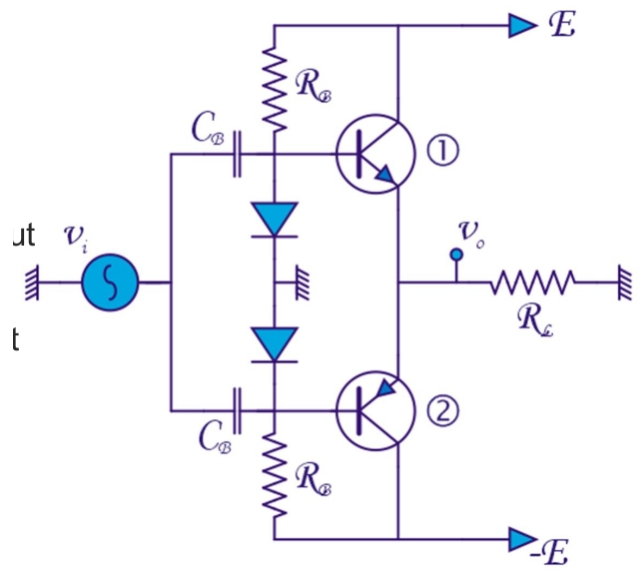
\includegraphics[width=8cm]{figures/ch09/pushpull2.jpg}
	\captionof{figure}{}
	\label{fig:pushpull2}
\end{minipage}
If $v_i$ is zero, both transistors carry the same current because of the symmetry, and hence there is no current in the load: $i_{C1} = i_{C2}$ and $i_{RL} = i_{C1} - i_{C2} = 0$. If $v_i$ increases, $i_{C1}$ will increase and $i_{C2}$ will decrease. Consequently, $i_{RL} = i_{C1} - i_{C2} > 0$ and transistor \Circled{1} will "push" current into the load. On the other hand, if $v_i$ decrease, $i_{C2}$ increases and $i_{C1}$ decreases, and transistor \Circled{2} will "pull" current out of the load. Because both transistors are emitter followers, $v_o \approx v_i$ and $A_v \approx 1$. To reiterate: the goal is to deliver current, not to increase the gain.\\
The configuration in figure \ref{fig:pushpull1} is a class A amplifier because it has a bias circuit with two resistors. If we replace resistors $R$ with diodes as in figure \ref{fig:pushpull2}, we have the same pre-biasing circuitry as the class B amplifier in figure \ref{fig:classB5}. In this case, resistor $R_B$ biases the diode to prevent cross distortion.\\
A way to provide both voltage amplification and current, is by using this circuit as the output trap after an OPAMP as in figure \ref{fig:pushpull3}.\\
\begin{figure}[h!]
	\centering
	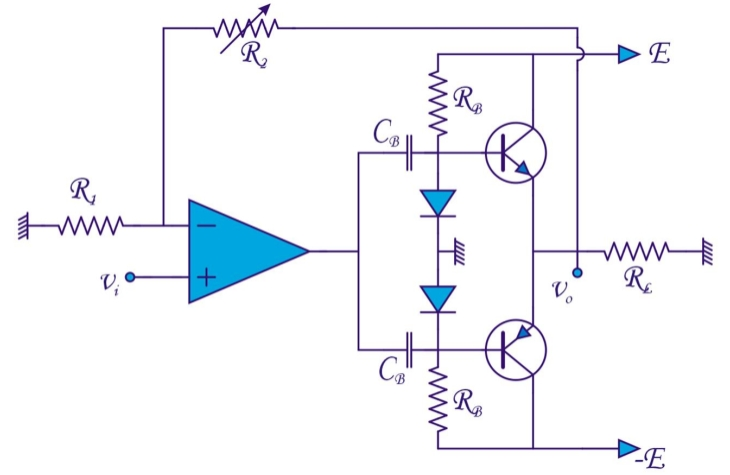
\includegraphics[width=8cm]{figures/ch09/pushpull3.jpg}
	\caption{Push-Pull amplifier with OPAMP}
	\label{fig:pushpull3}
\end{figure}
The voltage gain is set by the OPAMP: $A_v = 1 + \frac{R_2}{R_1}$. Note that the feedback via $R_2$ is applied to the output of the circuit, and not to the output of the OPAMP. Because of its high gain, the OPAMP will try to keep the votage $v$ between its two terminals equal to zero, so that we can write at the negative terminal:
$$
v_i = \frac{0/R_1 + v_o/R_2}{1/R_1 + 1/R_2} = \frac{R_1}{R_1 + R_2} v_o
$$
and this equation will set the output voltage. In this way, we avoid voltage loss through the push-pull stage.

\section{Class C Amplifier}
\label{sec:classC}
For the class C amplifier, we return to the circuit of the class A amplifier in figure \ref{fig:classA1}, but we now apply a negative bias (notice the orientation of $E_B$). This means that the transistor will conduct for only a fraction $2 \tau$ of the period $T$, as the waveform of $i_C$ in figure \ref{fig:classC2} shows.
\begin{minipage}{.5\textwidth}
	\centering
	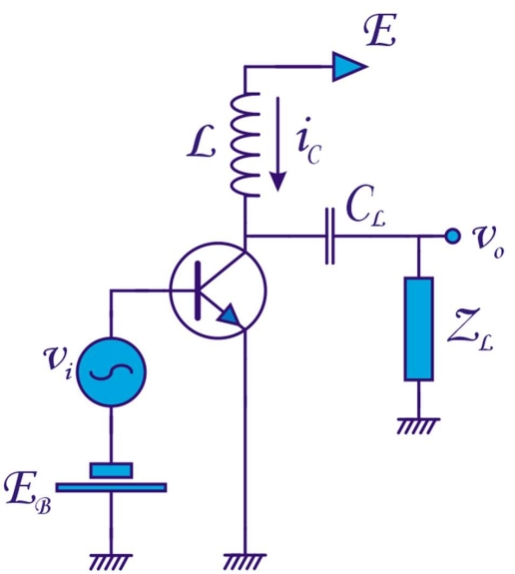
\includegraphics[width=6cm]{figures/ch09/classC1.jpg}
	\captionof{figure}{}
	\label{fig:classC1}
\end{minipage}%
\begin{minipage}{.5\textwidth}
	\centering
	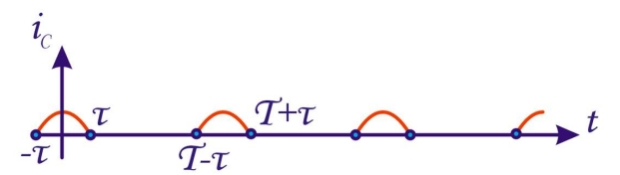
\includegraphics[width=8cm]{figures/ch09/classC2.jpg}
	\captionof{figure}{}
	\label{fig:classC2}
\end{minipage}
The current $i_C$ in figure \ref{fig:classC2} can be expressed as a cosine from which we subtract the lower $\cos(\omega_0 \tau)$ part:
$$
i_c = I_{cm} \frac{\cos(\omega_0 t) - \cos(\omega_0 \tau) }{1 - \cos(\omega_0 t)} \text{ if } kT - \tau < t < kT + \tau
$$
and $0$ elsewhere. Because this function is periodic, we can write it as a Fourier series i.e. the spectrum of the function:
$$
i_c(t) = I_0 + \sum_{n=1}^{\infty} I_n \cos(n\; \omega_0 t) \text{ with } I_n = \frac{2}{T} \int_{-T/2}^{T/2} i_c(t) \; \cos(n \omega_0 t) \; dt
$$
This spectrum is shown in figure \ref{fig:classC3}. From this spectrum, we only need the first harmonic, centered on $\omega = \omega_0$.\\

\begin{figure}[h!]
	\centering
	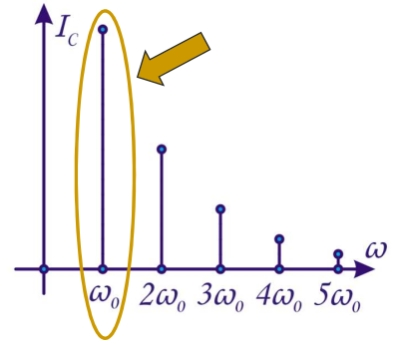
\includegraphics[width=6cm]{figures/ch09/classC3.jpg}
	\caption{Spectrum of figure \ref{fig:classC2}}
	\label{fig:classC3}
\end{figure}
The output voltage $v_o$ is equal to $v_o = Z_L \; i_c$. To just keep  the first harmonic, we need a $Z_L$ that is maximum at frequency $\omega_0 / 2\pi$, and zero at all other frequencies. This can be achieved by using an RLC tank as in figure \ref{fig:rlc} for $Z_L$. The impedance is:
$$
Z(\omega) = \frac{R}{1 + jQ \Big(\frac{\omega}{\omega_0} - \frac{\omega_0}{\omega}\Big)}
$$
with resonance pulsation $\omega_0 = \sqrt{1/LC}$ and quality factor $Q = \omega_0 RC = \omega_0/BW$ as in figure \ref{fig:rlc2}. So a proper choice of $L$ and $C$ determines $\omega_0$, and the choice of $R$ and $C$ sets the bandwidth. The bandwidth should be set by considering the bandwidth of the signals of interest, and by taking into account that non-linear distortion creates other harmonics.\\
How the expressions for the RLC circuit are found is explained in section \ref{sec:rlc}

\begin{minipage}{.5\textwidth}
	\centering
	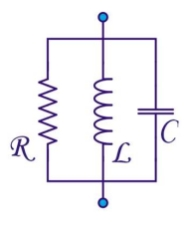
\includegraphics[width=4cm]{figures/ch09/rlc.jpg}
	\captionof{figure}{}
	\label{fig:rlc}
\end{minipage}%
\begin{minipage}{.5\textwidth}
	\centering
	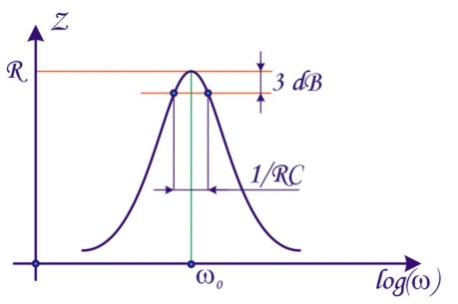
\includegraphics[width=8cm]{figures/ch09/rlc2.jpg}
	\captionof{figure}{}
	\label{fig:rlc2}
\end{minipage}

The class C amplifier has less dissipation in the transistor and higher power transfer. It is mostly used in telecommunication applications and high power transmission.

\subsection{The RLC Tank}
\label{sec:rlc}
Consider the parallel combination of a resistance $R$, a capacitance $C$ and an inductor $L$, as in figure \ref{fig:rlc}. Qualitatively, we see that if $\omega \ll \omega_0$, the inductance will act as a short circuit, and $Z \approx 0$. Similarly, if $\omega \gg \omega_0$, $C$ becomes a short and again $Z \approx 0$. Now let's analyze this circuit more formally.\\
Working with the admittances, we can write:
\begin{align*}
	Y &= \frac{1}{R} + j\omega C + \frac{1}{j\omega L} \\
	  &= \frac{j \omega L + R - \omega^2 RLC}{j\omega RL}
\end{align*}
and thus, for the impedance $Z$, where we use the resonance frequency $\omega_0^2 = \frac{1}{LC}$:
\begin{align*}
	Z(\omega) &=  \frac{j\omega LR}{j \omega L + R - \omega^2 RLC} = \frac{R}{1 - j\frac{R}{\omega L} + j\omega RC} \\
	  &= \frac{R}{1 + j(\omega RC - \frac{R}{\omega L})} = \frac{R}{1 + jRC (\omega - \frac{1}{\omega LC})}  \\
	  &=  \frac{R}{1 + jRC (\omega - \frac{\omega_0^2}{\omega})} = \frac{R}{1 + j\omega_0 RC \Big(\frac{\omega}{\omega_0} - \frac{\omega_0}{\omega}\Big)}
\end{align*}
If $\omega \ll \omega_0$ or if $\omega \gg \omega_0$, $Z \rightarrow 0$. If $\omega = \omega_0, \; Z(\omega_0) = R$. The impedance as function of frequency is plotted in figure \ref{fig:rlc2}. If we define the width where $Z = \frac{R}{\sqrt{2}}$ (i.e. a decrease of $-3$ dB) as the impedance bandwidth $\Delta \omega$, we can show that $\Delta \omega = \frac{1}{RC}$. This means that the resonance pulsation $\omega_0$ is controlled by $L$ and $C$, and the bandwidth is set by $R$ and $C$.\\
The quality factor is defined as the ratio between $\omega_0$ and the bandwidth:
$$
Q = \frac{\omega_0}{\Delta \omega} = \omega_0 \; RC
$$
With this expression, we can rewrite the expression for $Z$:
\begin{equation}
	Z(\omega) = \frac{R}{1 + jQ \Big(\frac{\omega}{\omega_0} - \frac{\omega_0}{\omega}\Big)}
	\label{eq:RLC_Z}
\end{equation}

\section{Class D Amplifier}
Figure \ref{fig:classD1} shows the circuit of a class D amplifier. This amplifier uses switches: when the top switch is open, the one in the bottom is closed, and vice versa. This can be implemented with two MOS transistors, as in figure \ref{fig:classD2}: a PMOS at the top and an NMOS at the bottom. when the input is high, the $v_{GS}$ of the bottom transistor is high and it will conduct and pull the output to the ground. When the input is low, the top transistor will conduct and pull the output to the supply $E$. These circuits will be studied in more detail in chapter \ref{ch:digital}.

\begin{minipage}{.5\textwidth}
	\centering
	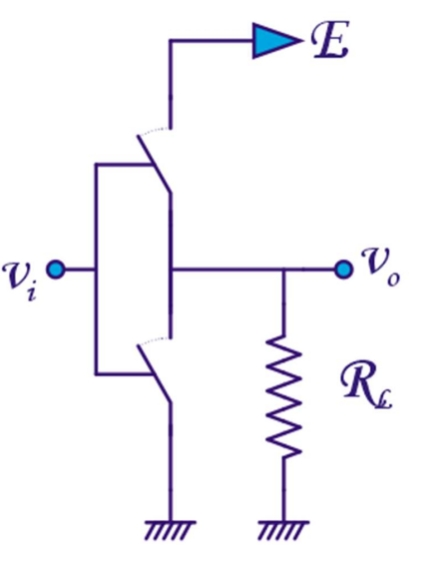
\includegraphics[width=4cm]{figures/ch09/classD1.jpg}
	\captionof{figure}{}
	\label{fig:classD1}
\end{minipage}%
\begin{minipage}{.5\textwidth}
	\centering
	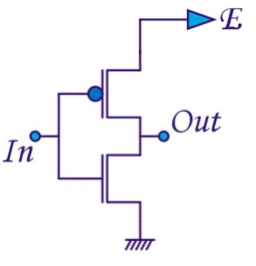
\includegraphics[width=4cm]{figures/ch09/classD2.jpg}
	\captionof{figure}{}
	\label{fig:classD2}
\end{minipage}

The advantage of a switch is that it never dissipates power: one of the switches will always be open, so no bias current can flow. In reality however, each of these switches (transistors) will have a parasitic resistor: each transistor will consume - when closed - a power $P_C$ because it will operate in the linear region (see \ref{sec:MOS_IV}) and we can model it as a (small) resistor $r_{ds}$ in series with $R_L$:
$$
P_C = i_{ds} \; v_{ds} = \frac{E}{r_{ds} + R_L} \frac{r_{ds} E}{r_{ds} + R_L} = E^2 \frac{r_{ds}}{(r_{ds} + R_L)^2} \approx E^2 \frac{r_{ds}}{R_L^2}
$$
The issue with this amplifier is that the amplitude is not preserved, so we can only transmit signals where the information is not encoded in the amplitude, but for example in the pulse width (pulse width modulation - PWM) or in the frequency (frequency modulation - FM).\\
If the load is not a resistor but a pure capacitor, i.e. if we replace $R_L$ by $C_L$, we can compute the associated power dissipation. When the top switch closes and the bottom one is open, a charge $Q = C_LE$ is transferred from the supply to the capacitance $C_L$. When the bottom switch is closed, the capacitor will discharge and the same amount of charge is transferred to ground. If this happens with a frequency $f$, we generate an effective current $i_{cap}$ equal to $fC_LE$. The average power consumption over one period is thus:
$$
P_{cap} = i_{cap} \; E = fC_L E^2
$$

\section{Class S Amplifier}
\label{sec:classS}
A class D amplifier can not be used when the signal amplitude is important, as in AM modulation. However, we can modify a class D amplifier to obtain a class S amplifier that is capable of amplifying AM signals.\\
\begin{figure}[h!]
	\centering
	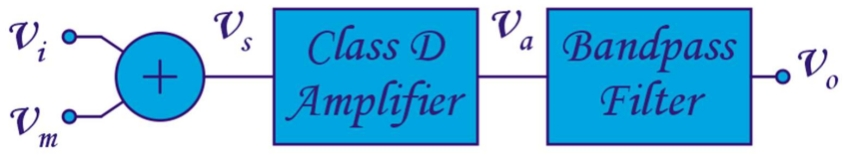
\includegraphics[width=11cm]{figures/ch09/classS1.jpg}
	\caption{Block diagram of a class S amplifier}
	\label{fig:classS1}
\end{figure}

To do this, we first take the sum of the input signal $v_i$, which we assume has the form $v_i = A(t) \cos(\omega_0 t)$, with a signal $v_m = \cos(\frac{\omega_0}{2} t)$. We assume that $|A(t)| \ll 1$, so that $|v_m| \gg |v_i|$. By representing these signal as Fresnel vectors as in figure \ref{fig:classC1}, with $v_m$ in red, $v_i$ in green and $v_s = v_i + v_m$ in yellow, we see the small green arrow $v_i$ rotates fast around the slowly rotating red arrow $v_m$. By tracing out the end-points of the green arrow $v_i$, we see that the amplitude information $A(t)$ of $v_i$ is new encoded in the phase of $v_s$. We can now use a class D amplifier to amplify the signal, losing all amplitude information but keeping the phase information intact, and extract the amplitude information from the output signal with a bandpass filter, as in figure \ref{fig:classS1}.\\

\begin{figure}[h!]
	\centering
	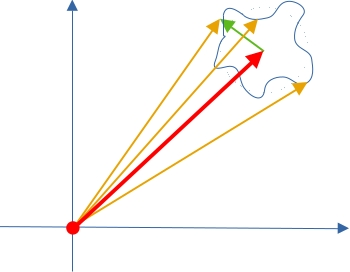
\includegraphics[width=8cm]{figures/ch09/classS2.jpg}
	\caption{}
	\label{fig:classS2}
\end{figure}

Mathematically, we can write:
\begin{align*}
	v_s &= A(t) \cos(\omega_0 t) + \cos(\frac{\omega_0}{2} t) = A(t) \cos(\frac{\omega_0}{2} t) \cos(\frac{\omega_0}{2} t) - A(t)  \sin(\frac{\omega_0}{2} t) \sin(\frac{\omega_0}{2} t) + \cos(\frac{\omega_0}{2} t) \\
		&= [1 + A(t) \cos(\frac{\omega_0}{2} t)] \cos(\frac{\omega_0}{2} t) - [A(t) \sin(\frac{\omega_0}{2} t)] \sin(\frac{\omega_0}{2} t) \\
		&= \sqrt{[1 + A(t) \cos(\frac{\omega_0}{2} t)]]^2 +  [A(t) \sin(\frac{\omega_0}{2} t)] ^2} \cos[\frac{\omega_0}{2} t + \arctan \frac{A(t) \sin(\frac{\omega_0}{2} t)}{1 + A(t) \cos(\frac{\omega}{2} t)}]
\end{align*}
Because we lose the amplitude, the output of the class D amplifier $v_a$ is equal to:
\begin{align*}
	v_a = K \cos[\frac{\omega_0}{2} t + \arctan \frac{A(t) \sin(\frac{\omega_0}{2} t)}{1 + A(t) \cos(\frac{\omega}{2} t)}]
\end{align*}
with $K$ the gain of the amplifier. When we take into account that $|A(t)| \ll 1$, we can simplify this expression:
\begin{align*}
	v_a &= K \cos[\frac{\omega_0}{2} t + \arctan \frac{A(t) \sin(\frac{\omega_0}{2} t)}{1 + A(t) \cos(\frac{\omega}{2} t)}] \approx K \cos[\frac{\omega_0}{2} t + \arctan A(t) \sin(\frac{\omega_0}{2} t)] \\
		&\approx K \cos[\frac{\omega_0}{2} t + A(t) \sin(\frac{\omega_0}{2})] = K \cos(\frac{\omega_0}{2} t) \cos[A(t) \sin(\frac{\omega_0}{2} t)] - K \sin(\frac{\omega_0}{2} t) \sin[A(t) \sin(\frac{\omega_0}{2} t)] \\
		&\approx K \cos(\frac{\omega_0}{2} t) - KA(t) \sin^2(\frac{\omega_0 t}{2} t) \\
		&\approx K \cos(\frac{\omega_0}{2}t) - \frac{K}{2} A(t) + \frac{K}{2} A(t) \cos(\omega_0 t)
\end{align*}
After the bandpass filter, centered on $\omega_0$, the output signal becomes:
$$
v_o \approx \frac{K}{2} A(t) \cos(\omega_0 t)
$$
We have thus amplified with high efficiency, and conserved the amplitude $|A(t)|$.

\section{The Selective Amplifier}
\label{sec:selective_amp}
Until now, we have amplified a relatively large bandwidth, and we have made no effort to restrict the amplification only to a specific frequency. In most telecommunications applications however, we are often only interested in a specific segment of the spectrum. This means we want to amplify a narrow bandwidth around the center frequency $\omega_0$, and discard all other frequencies.\\
A perfect solution for this would be to use the RLC-circuit from section \ref{sec:rlc}, which has as impedance the resistor $R$ at resonance and zero impedance elsewhere as in figure \ref{fig:rlc2b}. However, in reality every inductance $L$ also has a small series resistance $r_s$. We want to replace this series combination of an ideal $L$ with a parasitic $r_s$ with a parallel combination of $L$ with a resistance $R_p$ as indicated in figure \ref{fig:selective1}.\\

\begin{minipage}{.5\textwidth}
	\centering
	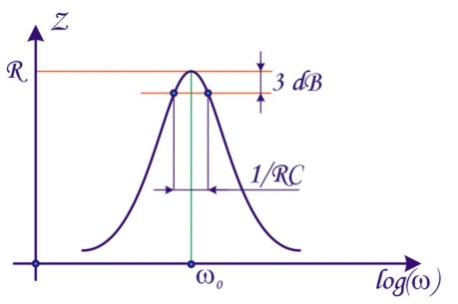
\includegraphics[width=7cm]{figures/ch09/rlc2.jpg}
	\captionof{figure}{}
	\label{fig:rlc2b}
\end{minipage}%
\begin{minipage}{.5\textwidth}
	\centering
	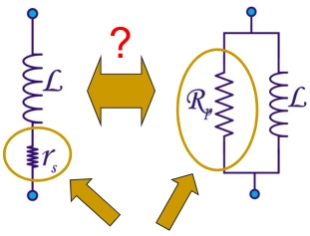
\includegraphics[width=5cm]{figures/ch09/selective1.jpg}
	\captionof{figure}{}
	\label{fig:selective1}
\end{minipage}
The impedance of an inductor $L$ in series with a resistor $r_s$ is:
\begin{align*}
	Z_{L + r_s} &= j \omega L + r_s \\
	\frac{1}{j \omega L + r_s} &= \frac{r_s - j \omega L}{r_s^2 + \omega^2 L^2} \\
		&\approx \frac{r_s}{\omega^2 L^2} + \frac{1}{j\omega L}
\end{align*}
This last simplification is only valid if $\omega L \gg r_s$, or in other words, if the quality factor of the coil (the inductor) $Q_C = \frac{\omega L}{r_s}$ is a lot larger than $1$. This means that we have an equivalent impedance consisting of a resistor $R_p = \frac{\omega^2 L^2}{r_s}$ in parallel with an inductance $j\omega L$.\\
When we add a capacitor in parallel with $R_p$ and $L$, we get a true RLC-tank as in figure \ref{fig:rlc} - but in reality we have a non-ideal coil in parallel with $C$. The quality factor of the whole is $Q = \omega R_p C = \frac{R_p}{\omega_0 L} = Q_C$. So any LC-combination has in reality an impedance as in figure \ref{fig:rlc2b}, but with a maximum of $R_p = \frac{\omega^2 L^2}{r_s}$ and a bandwidth of $\frac{1}{R_p C}$.\\
In a real RLC-circuit, we can push the resistance $r_s$ to become a resistance $R_p$ in parallel with the true resistance $R$. The quality factor if the entire circuit is $Q = \omega_0 (R_p || R) C <  \omega_0 R_p C = Q_C$. So the use of an external resistor decreases the quality factor.\\

\begin{figure}[h!]
	\centering
	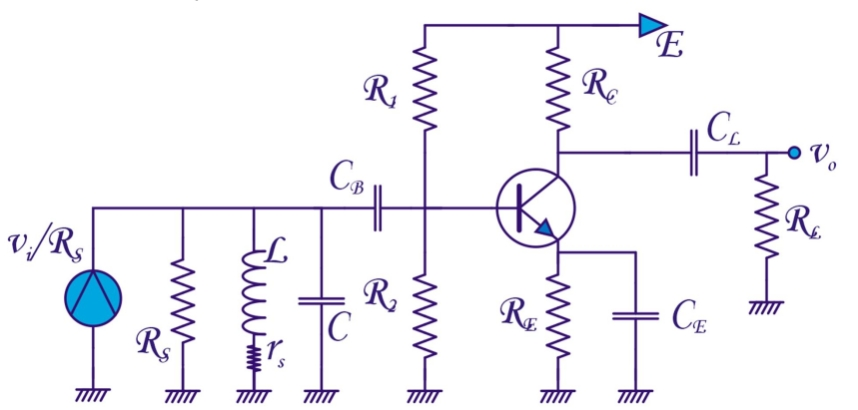
\includegraphics[width=10cm]{figures/ch09/selective2.jpg}
	\caption{}
	\label{fig:selective2}
\end{figure}
To construct a selective amplifier, we add the LC-circuit to the input stage of a common-emitter amplifier, as in figure \ref{fig:selective2}. Note how the input has been replaced by the Norton equivalent, namely $Z_N = R_S$ and $I_N = v_i/R_S$. \\
To compute the central frequency and gain, we introduce the small-signal equivalent circuit in figure \ref{fig:selective3}, where we suppose that both $C_B$ and $C_E$ are short circuits, i.e. we are in the normal operating domain, and $C_L$ is also a short circuit.\\
\begin{figure}[h!]
	\centering
	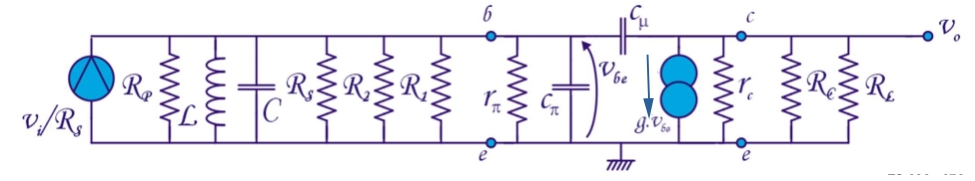
\includegraphics[width=14cm]{figures/ch09/selective3.jpg}
	\caption{The selective amplifier}
	\label{fig:selective3}
\end{figure}
We can simplify the circuit in figure \ref{fig:selective3} by replacing $C_\mu$ by the Miller capacitance $C_M = (1 + g R_{eq}) C_\mu$, by introducing an equivalent resistance $R_{eq} = r_c || R_C || R_L$ and by grouping all resistors at the left side together: 
$$R_\pi = R_p || R_s || R_1 || R2 || r_\pi$$
The resulting circuit is shown in figure \ref{fig:selective4}. The RLC tank is formed by $R_\pi$, $C_\pi$ and $L$, so the central frequency $\omega_0$ is $\frac{1}{\sqrt{LC_\pi}}$ and the bandwidth $\Delta \omega = \frac{1}{R_\pi C_\pi}$. At $\omega_0$, the  impedance at the input is $Z = R_\pi$.\\
To compute the gain, we observe that $v_{be} = \frac{v_i}{R_S} R_\pi$ - if $R_S$ is very small, this reduces to $v_{be} \approx v_i$ - and the output voltage is:
$$
v_o = - R_{eq} \; g \; \frac{v_i}{R_S} R_\pi
$$
This is only valid at $\omega = \omega_0$ and so the gain is $A_v = - g \frac{R_\pi}{R_S} R_{eq}$. At frequencies $\omega < \omega_0 - \Delta \omega$ or $\omega > \omega_0 + \Delta \omega$ the gain is (almost) zero.
\begin{figure}[h!]
	\centering
	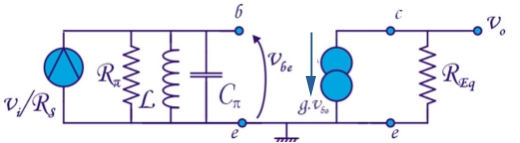
\includegraphics[width=12cm]{figures/ch09/selective4.jpg}
	\caption{}
	\label{fig:selective4}
\end{figure}

